\documentclass[24pt]{article}
\usepackage[left=2cm,right=2cm,top=2cm]{geometry}
\usepackage{physics}
\usepackage{graphicx}
\usepackage{setspace}
\usepackage{amsfonts}
\usepackage{amsmath}
\usepackage{biblatex}
\usepackage[toc,page]{appendix}

\onehalfspacing

\begin{document}


\begin{titlepage}
\textbf{\begin{center}
{\huge Investigation of the Magnetic Properties of $RNiO_3$}
\end{center}}


\begin{figure}[h!]
\centering
	
\includegraphics[width=0.4\textwidth]{julogo.png}
	
\end{figure}
	\begin{center}
	\begin{huge}
	\textbf{Sahil Islam}\\
	\end{huge}
\begin{LARGE}
Exam Roll No: MPHD\\
Class Roll No: 001820702023\\
Registration No:133-136 of 2015-2016\\

Department of Physics\\

Jadavpur University\\

\vspace*{\fill}
\textbf{A project submitted for the final semester of\\
 Master of Science\\
2020}\\

\end{LARGE}		
	\end{center}
\end{titlepage}



\newpage

\title{\textbf{{\large \begin{center}
Acknowledgements
\end{center}}}}
\date{}
\author{}
\maketitle

\begin{large}
The project work included in the dissertation could not have been performed if not for the assistance, patience and support of many individuals. I would like to extend my gratitude first and foremost to my advisor Prof. Ajay Kumar Ghosh for mentoring me over the course of my research work with his valuable guidance, constructive criticism and continuous encouragement. I must acknowledge the support of Souvik Haldar for his valuable suggestions, inputs and encouragements throughout the work. 
    I gratefully acknowledge the Department of Physics, Jadavpur University for providing the necessary resources to complete this work.
    To the end, I express my deepest sense of gratitude to my family members who always provided major inspiration and silent support to pursue my whole academic career. \\
\end{large}

\begin{flushleft}
\begin{large}
Department of Physics\\	
Jadavpur University\\
Jadavpur, Kolkata-32\\
Date- 10/09/2020\\
\end{large}
\end{flushleft}

\begin{flushright}
{\large Sahil Islam}
\end{flushright}

\newpage
\tableofcontents
\newpage


\title{{\LARGE \textbf{Investigation of the magnetic properties of \textbf{$RNiO_3$}}}}
\author{}
\date{}
\maketitle
\begin{abstract}


 In this project we probed into the magnetic properties of the compounds like $RNiO3$($R$=Rare earth elements). The magnetic properties are believed to be controlled by $NiO_6$ octahedra. These kind of compounds generally has an  orthorhombically distorted pervoskites. We tried to solve the Ising Hamiltonian of this particular structure using Mean Field Approximation.From the canonical ensemble partition function we calculated the magnetization per spin and total magnetization and from that  investigated the magnetic property (behaviour of magnetization with varying temperature and varying external field) of the $NiO_6$ octahedra. Here for simplicity we worked with a single $NiO_6$ octahedra.\\
 We observed that saturation magnetization is observed for all temperatures and the low temperature polarized spins breaks the orientation as temperature is increased. From susceptibility-temperature curve we verified that the substance is paramagnetic in nature. \\


\end{abstract}


\section{{\Large Introduction}}
{\large The magnetic properties like Magnetization, Susceptibility, Phase Transition etc. are very interesting and also a quite difficult to explain phenomenons in terms of Statistical Mechanics. There are various kind of crystals which shows phase transitions at various temperatures. To explain the behaviour of a metal near critical temperature, to observe the nature of magnetization, energy, specific heat or the magnetic susceptibility of a substance with various temperature and external filed parameters, we use some models to explain those theoretically. One of those models is Ising Model. This model was proposed by Ernst Ising initially to explain those behaviours in one dimension. He believed this model fails for higher dimensions. But later Lars Onsager proposed a complicated but very nice solution to the two dimensional Ising Model proving that this model can be useful in more than one dimensions. But proper analytic solution of this in 3D is not yet available. In 3D, this is done by some more approximations like Mean Field Theory or computationally using Monte Carlo Method etc.   \\ 
$LaNiO_3$ is a very interesting and useful material having usage as metallic bottom electrodes in various ferroelectric and superconductor related devise. It displays a metallic like behaviour and Pauli Paramagnetism for a wide range of temperature.\\}

\subsection{{\large \textbf{The Ising Model}}}

\subsubsection{\large \textbf{Hamiltonian}}

\begin{large}

In this Model we consider $N$ sites of a $d$-dimensional lattice where each lattice site consists of spins(i.e. magnetic moments). Physical phenomenons like magnetic moments, susceptibility, specific heat etc. are explained in this model by considering the interactions between the spins. The simplest case is considering only the nearest  neighbour interactions. The Hamiltonian of the system depends on the interactions of the spins and an exchange integral term($J$) which has the dimension of energy. If we write the eigenvalue of the $i^{th}$ spin as $s_i$, then the Hamiltonian will be,

\begin{equation}
\mathcal{H}(s_1,s_2,...s_N)=-J \sum_{{\small nearest.neighbours}} s_i s_j 
\end{equation}


If $J>0$ the neighbouring spins prefer to be aligned (i.e. $ \uparrow \uparrow$ or $ \downarrow \downarrow$). Such a spin system is called ferromagnet. And for $J<0$, neighbouring spins are anti-aligned($\uparrow \downarrow$), these are called anti-ferromagnet.  \\
In presence of an external magnetic field $H$, this Hamiltonian takes the form:

\begin{equation}
\mathcal{H}(s_1,s_2,...s_N)=-J \sum_{nearest.neighbour} s_i s_j - H \sum_{i} s_i
\end{equation}

\end{large}

\subsubsection{{\large \textbf{Periodic Boundary Condition}}}
{\large To solve this model we use an assumption called periodic boundary condition. This assumes, say in one dimension, the $(N+1)^{th}$ spin is the $1^{st}$ spin again. Which makes the whole oneD lattice like a ring. And in twoD this assumption makes the  lattice sheet a torus. This assumptions makes the model easier to solve in both oneD and twoD. Though it my not be the most realistic case to work with, but the results obtained by taking assumption never showed very wrong results rather it gives good idea of the system. But in three dimensional case we can use another assumption called \textit{The Mean Field Approximation } to solve the system.\\}

\subsubsection{{\large \textbf{Mean Field Approximation}}}
{\large In the mean field approximation, the basic assumption is that instead of interacting directly with the neighbouring spins, each spin interact with each other with a 'mean field' which follows from the mean orientation of the neighbouring spins.\\
Here for the term in the Hamiltonian $s_i s_j$, we write

\begin{equation}
s_i s_j = [(s_i - m)+m][(s_j - m)+ m] ...(3),
\end{equation}

here $m$ is the mean field that the spins interact with. Thus,

\begin{equation}
s_i s_j  = (s_i - m)(s_j - m) + m(s_j - m) + m(s_i - m)+ m^2
\end{equation}
 


Here we identify, $(s_i - m)$ and $(s_j - m)$ are the fluctuations of the individual spins from the mean field. Though these fluctuations for individual spins may not be small but the product fluctuations of two different neighbouring spins  may be neglected while doing the sum $\sum_{n.n}$.\\
Thus, the Hamiltonian becomes:

$$\mathcal{H}_{m.f} = -J \sum_{n.n} [m (s_i - m) + m (s_j - m)] - H \sum_{i} s_i
$$
\begin{equation}
\implies \mathcal{H}_{m.f} = \frac{1}{2} J N q m^2 - (J q m + H)\sum_{i} s_i
\end{equation}

Here $N$ is the total number of lattice sites and $q$ is the number of nearest neighbours. The $\frac{1}{2}$ comes because we do the sum over pairs not on the individual sites.\\
Thus if we see the new mean field Hamiltonian carefully, we see that it has removed the interactions and an effective magnetic filed is in action:

\begin{equation}
H_{eff} = H + J q m. 
\end{equation}

From here, in \textit{Canonical Ensemble}, we can write a partition function,

\begin{equation}
Z= \sum_{s_i} \exp[-\beta \mathcal{H}(s_i)]
 \end{equation}

Here $\beta = \frac{1}{k_B T}$, where, $k_B$ is the Boltzman Constant.\\

And the average magnetization:

\begin{equation}
m= \frac{1}{N} \sum_{i} s_i = \frac{1}{N \beta} \pdv {log(Z)}{H}
\end{equation}

This is the core concept of the mean field theory. Here we will try to solve the Hamiltonian i.e. try to write the partition function for a specific kind of lattice, and calculate some properties like magnetization, specific heat etc. Following the standard calculation procedure\footnote{For detailed calculation see Appendix A} we can write the magnetization per spin as: \\
\begin{equation}
m = \tanh(\beta H_{eff})
\end{equation}


And, the total magnetization ($M$) is given by the sum of all $m$-s.\\
And, the susceptibility is,\\
\begin{equation}
\chi = (\pdv{M}{H})_{T}
\end{equation}

Now, let's know about the sample.\\}

\subsection{\textbf{{\large The Sample}}}
\subsubsection{\large  \textbf{Crystal Structure}}
{\large The sample we are working with is generally denoted by $RNiO_3$ perovskites. Here $R$ is rare earth elements.This kind of materials has a structure of orthorhombically distorted perovskites. The ideal cubic structure of $R$ and $Ni$ has a 3D array of  corner sharing $Ni O_6$ octahedra.}

\begin{figure}[h!]
\centering
	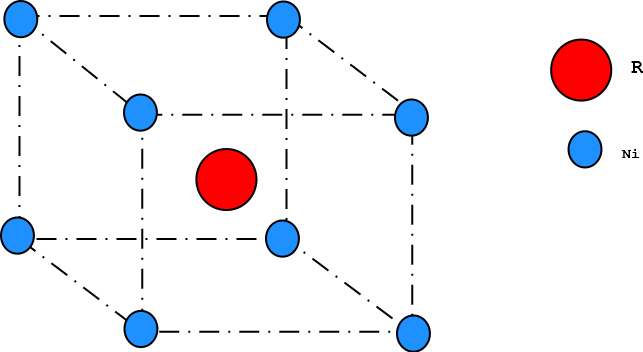
\includegraphics[width=0.4\textwidth]{RNiO3_2.png}
	\caption{The basic Cubic Structure without the Oxygen}
	\end{figure}
	
Figure 1 shows the basic ideal cubic structure where at the centre there is an $R$ and all the corners have $Ni$ in it.
\begin{figure}[h!]
\centering
	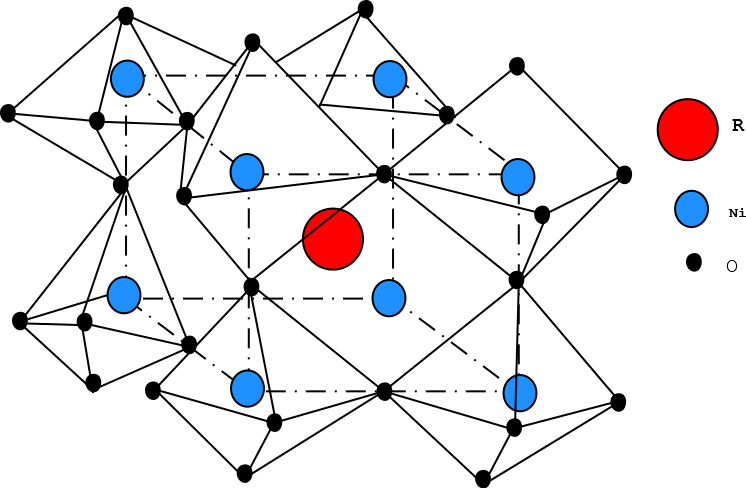
\includegraphics[width=0.4\textwidth]{RNiO3.png}
	\caption{The Ideal Perovskite Structure }
	\end{figure}
	
\begin{figure}[h!]
\centering
	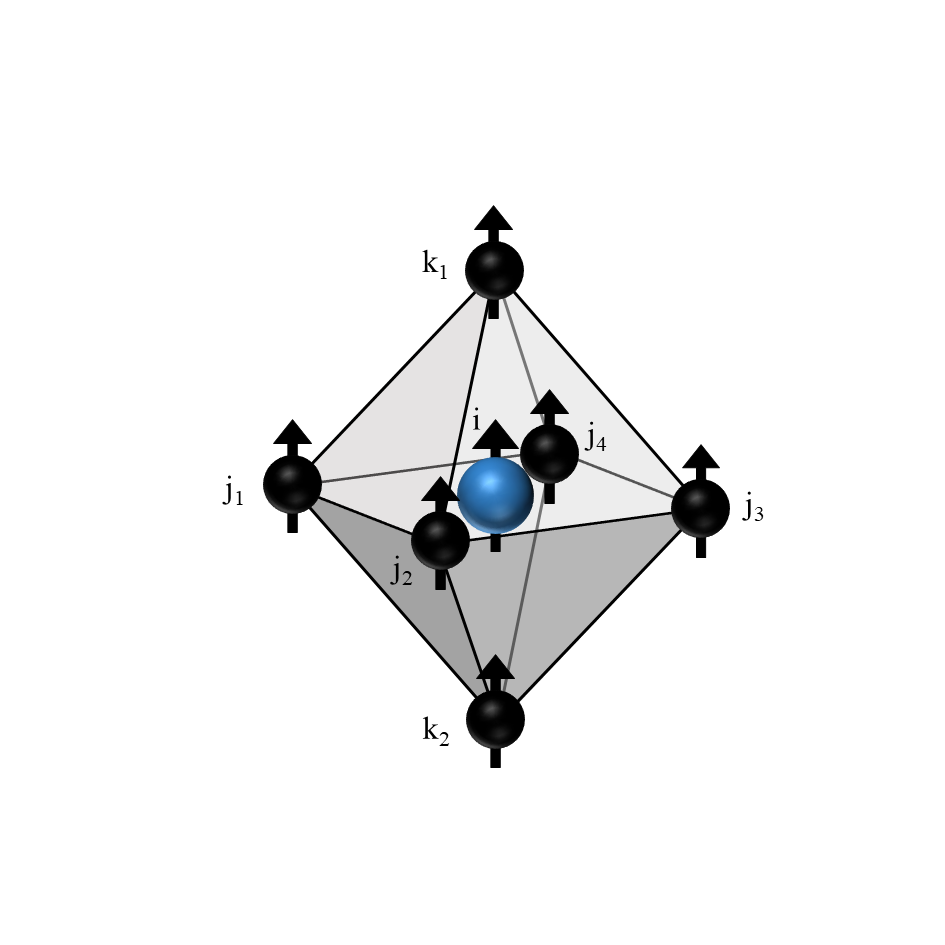
\includegraphics[width=0.4\textwidth]{NiO3.png}
	\caption{Structure of $NiO_6$ octahedra. Black spheres are O-ions and blue sphere is Ni-ion. Ni-ion is at the center of a BCC position, and O-ions are at the FCC positions.}
	\end{figure}
	
The $Ni$-s at the corners have 6 $O$-s around it (Figure 2). This makes it a $NiO_6$ structure, but Oxygens are shared by the Nickels resulting the whole structure to be $RNiO_3$.\\

\subsubsection{{\large \textbf{Spin Structure}}}
\begin{large}
Generally while solving the Ising Model we take the spins of the lattice points as $\pm1$ , but in case of real crystals like this we can have a mixed spin structures. Here we will take spins of $LaNiO_3$ which belongs to the class of $RNiO_3$.\\
We know that the term symbols for $Ni$, $O$ and $La$ are $^3F_4$, $^3P_2$ and  $^2D_{\frac{3}{2}}$ respectively. Thus their spins are $\pm 1$, $\pm 1$ and $\pm\frac{1}{2}$ respectively. As previously said, the $NiO_6$ octahedra (Figure 3) is primarily responsible for the magnetization of the $RNiO_3$ system, we will try to write down the Hamiltonian associated with it.\\
\end{large}

\section{{\Large Formulation}}
\subsection{\large \textbf{Hamiltonian}}
\begin{large}
The Hamiltonian of the system(Figure 3) in presence of external magnetic field $\vec{H}$ reads,

$$
\mathcal{H} = - \frac{1}{2} \sum_{m=1}^{4}J_{i j_{m}} (\vec{S_i}.\vec{S_{j_m}})
- \frac{1}{2} \sum_{n=1}^{2}J_{i k_{n}} (\vec{S_i}.\vec{S_{k_n}})
- \frac{1}{2} \sum_{p=1}^{4} \sum_{\substack{q=1\\ q \neq p}}^{4}J_{j_{p} j_{q}}(\vec{S_{j_{p}}}. \vec{S_{j_{q}}})
$$
\begin{equation}
- \frac{1}{2} \sum_{r=1}^{4}J_{j_{r} k_{1}} (\vec{S_{j_r}}.\vec{S_{k_1}})
- \frac{1}{2} \sum_{r=1}^{4}J_{j_{r} k_{2}} (\vec{S_{j_r}}.\vec{S_{k_2}})
- \vec{H}.\vec{S_i} - \vec{H}. \sum_{t=1}^{4}\vec{S_{j_t}} 
-\vec{H}. \sum_{u=1}^{2}\vec{S_{k_u}}
\end{equation}


Here, $J_{i {j_m}}, J_{i k_{m}} and J_{j_p j_q}$ represents the  exchange interactions between two  spin sites indicated by the indices used. Here we have considered only the nearest neighbour and next to nearest neighbour interaction. So, we ignored the interactions between two apex spins($k_1, k_2$) and corner spins of the square plane(i.e. $(j_2,j_4) and (j_1, j_3)$).
\end{large}

\subsection{{\large \textbf{Magnetization and Susceptibility}}}
\begin{large}


Now from equation (6) and (9), we can write,

\begin{equation}
m_i = \tanh{\beta (3 J_1 m_l)}
\end{equation}
and

\begin{equation}
m_l = \tanh(\beta (3 J_1 m_i + 6 J_2 m_l))
\end{equation}

Here $m_j = m_k = m_l$ and
 $J_1 = J_{ij}=J_{i_k}$ is the exchange integral between one $Ni$ and one $O$ atom and 
 $J_2$ is the same for two $O$ atoms.\\
 
 Now, our system has 7 spins. 6 $O$ spins and one $Ni$ spin. Thus, the total magnetization will be,\\
 $$M = m_i+ m_{j_1} + m_{j_2}+ m_{j_3}+ m_{j_4}+ m_{k_1}+ m_{k_2} $$
 
\begin{equation}
\Rightarrow M = 6 m_l + m_i
\end{equation}
\\Thus, the final form of magnetization will be,\\
\begin{equation}
M = \tanh{\beta (3 J_1 m_l)} + 6 \tanh(\beta (3 J_1 m_i + 6 J_2 m_l))
\end{equation}

And from equation(10) we calculate , the susceptibility to be,

\begin{equation}
\chi = \frac{3 J_1 m_l ' + 1}{k_B T \cosh[2](\frac{3J_1 m_l + H}{k_B T})}+ 6 \frac{3 J_1 m_i '+ 6}{k_B T \cosh[2](\frac{J _1 m_i + 6 J_2 m_l + 6 H} {k_B T })- 6 J_2}
\end{equation}

We will plot these, and study their nature.\\
\end{large}

\section{{\Large Results}}

{\large To plot those equations numerically, we took $k_B =1 $, $J_1 = 1$ and $J_2 = 0.5$.}\footnote{The numerical values seen in the graphs are taken such as the nature of the curves can be seen. These values will not match with any real data. }  


\subsection{\large \textbf{Magnetization Curve}}

\begin{large}
Putting those values in equation (15) we get,\\
\begin{equation}
M = \tanh[\frac{1}{T}(3 m_l +H)]+ 6 \tanh[\frac{1}{T}(3 m_i + 3 m_l + 6 H)]
\end{equation}
\end{large}
\begin{figure}[h!]
\centering
	\includegraphics[width=0.6\textwidth]{MagnetizationVs Field.png}
	\caption{Variation of Magnetization with Field at different Temperatures}
	\end{figure}

\begin{figure}[h!]
\centering
	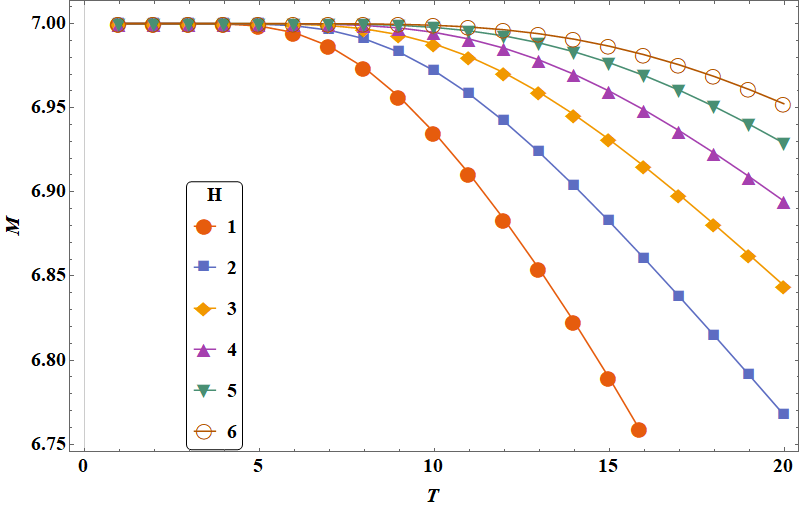
\includegraphics[width=0.6\textwidth]{Magnetization-Temperature.png}
	\caption{Variation of Magnetization with Temperature at different Fields with $k_B =1, J_1 = 1, J_2 = 0.5$}
	\end{figure}

\subsection{\large \textbf{Susceptibility Curve}}
From equation (16), if we put $J_1=1$, $J_2=0.5$ and $k_B =1$, we get,
$$
\chi = \frac{3 m_l '+1}{T \cosh[2](\frac{3 m_l + H}{T})} + 6 \frac{3 m_i '+ 6}{T \cosh[2](\frac{m_i + m_l + 6 H}{T})-3}
$$
 The plot is shown in figure(6).
 
\begin{figure}[h!]
\centering
	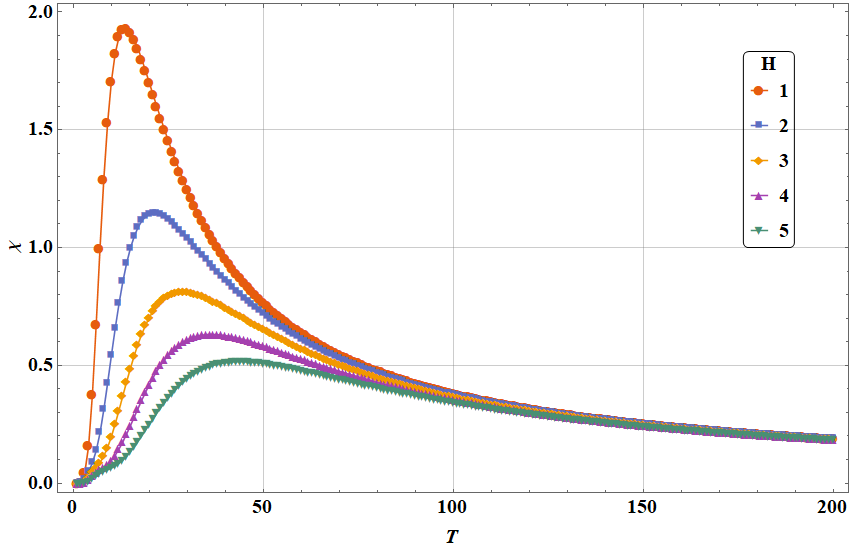
\includegraphics[width=0.6\textwidth]{Susceptibility Vs Temperature.png}
	\caption{Variation of Susceptibility with Temperature at different Fields with $k_B =1, J_1 = 1, J_2 = 0.5$}
	\end{figure}
 
\newpage

\section{{\Large Discussions}}

\begin{large}
\begin{itemize}


\item In the $M-H$ curve(Figure 4), the saturation magnetization is observed for all the temperatures. As the temperature increases, the thermal energy of the spins increases, therefore higher field is required to polarize all the spins in a particular direction.\\
\item In the $M-T$ curve(Figure 5), we see that magnetization asymptotes to a particular value for any given field. Which indicates in low temperature the given external magnetic filed is dominated by the temperature parameters. At low temperatures that asymptotic value of the magnetization indicates higher internal energy.  But as we increase the temperature, the internal energy increases and the external field starts affecting the system. 
In lower value of the temperature, the spins are polarized at a particular direction which gives rise to that particular asymptotic value of magnetization.  After applying very small field, as temperature is being increased, the orientation of the spins breaks and the magnetization decreases monotonically with temperature. As we apply higher fields, more temperature is required to break the orientation of the spins.\\
\item In the $\chi - T$ curve, we see that there is no discontinuity  in the curve. This clearly indicates, the structure we worked with is paramagnetic in nature. At low temperatures, the susceptibility increases with temperature upto a certain value, then decreases rapidly. At low temperature, the spins are aligned,  so they produce a higher magnetization value that leads to increase susceptibility. But after a certain temperature, the spins become randomly oriented which leads to rapid decrease in $\chi$. As the field is increased we see that the curve flattens so the peak value of $\chi$ decreases. 

\end{itemize}
\end{large}

\begin{thebibliography}{9}

\bibitem{Reif}
Fundamentals of Statistical and Thermal Physics. F. Reif. Levant Press. 1st Indian edition 2010.

\bibitem{Huang}
Statistical Mechanics, 2nd Edition, Kerson Huang, Wiley India Pvt. Limited, September 2008.

\bibitem{Tong}
Statistical Physics. 
University of Cambridge Part II Mathematical Tripos, 
David Tong.
http://www.damtp.cam.ac.uk/user/tong/statphys.html

\bibitem{article}
Structural, magnetic and electronic properties of $RNiO_3$ perovskites (R = rare earth).
Mar´ıa Luisa Medarde
Laboratory for Neutron Scattering, Switzerland. 
Received 17 July 1996, in final form 14 October 1996

\bibitem{Guan}
Electronic structure and optical properties of $LaNiO_3$: First-principles calculations
Li Guan, Baoting Liu, Litao Jin, Jianxin Guo, Qingxun Zhao, Yinglong Wang, Guangsheng Fu
College of Physics Science and Technology, Hebei University, Baoding 071002, China

\end{thebibliography}

\newpage

\begin{appendices}

\section{Mean Field Calculation}
$$
Z = \sum_{s_i}\exp[-\beta \mathcal{H}(s_i)]
$$
Here,
$$
\mathcal{H}(s_i)= \mathcal{H}_{m.f}
$$
Thus,
$$
Z = \sum_{s_i}\exp[-\beta \mathcal{H}_{m.f}]
$$
Where, from equation $(5)$, 
$$
\mathcal{H}_{m.f} = \frac{1}{2} J N q m^2 - (J q m + H)\sum_{i} s_i
$$
Thus, 
$$
Z = e^{-\frac{1}{2} \beta J q m^2} \sum_{s_i}\exp[\beta H_{eff} \sum_i s_i] 
$$
Here $H_{eff} = H + J q m $;\\
Thus,

$$
Z =  e^{-\frac{1}{2} \beta J q m^2}\prod_{i}\sum_{s_i}\exp(\beta H_{eff} s_i)
$$ 

Here for both $Ni$ and $O$, the spins are $\pm 1$.\\
Thus for both of them we can write,

$$
Z =  e^{-\frac{1}{2} \beta J q m^2}\prod_{i}(\exp(\beta H_{eff})+ \exp(- \beta H_{eff}))
$$

Here the each term inside the product gives the same value. Thus the product becomes power.
$$
Z =  e^{-\frac{1}{2} \beta J q m^2}[\exp(\beta H_{eff})+ \exp(- \beta H_{eff})]^N
$$
Here N is the total number of spins. 
Therefore,
$$
Z = e^{-\frac{1}{2} \beta J q m^2} 2^N \cosh[N](\beta H_{eff})
$$

Now, 
$$
\log Z = -\frac{1}{2} \beta J N q m^2 + N \log 2 + N \log\cosh(\beta H_{eff})
$$
Thus, 
$$ \pdv{\log Z}{H} = N \beta \tanh(\beta H_{eff})
$$
Thus,
$$
m = \tanh(\beta H_{eff})
=> m = \tanh(\beta (H + J q m))
$$

From here we can calculate $\chi$ as,

$$
\pdv{m}{H}= \frac{\beta}{\cosh[2](\beta J q m)} (1+ J q \pdv{m}{H})
$$
Thus, 
$$
\chi = N \pdv{m}{H} = \frac{N \beta}{\cosh[2](\beta J q m)} (1+ \frac{J q}{N} \chi)
$$
\end{appendices}

\end{document}